\section{Task 2: Online Password Attack} \label{ch:pentesting:password}
An online password attack refers to probing an active login, as opposed to an offline attack where you for example might try to crack a hash of a leaked database. This attack involves using some type of approach to test many passwords of a login form to try and find valid credentials. The local web admin page (see section \ref{ch:system}) has a login page that could potentially be brute-forced.

\subsection{Background}
A password attack, or password cracking, refers to cyber-attacks where the attacker tries to figure out valid credentials, to gain authorized access to a system. These can be categorized into two groups: offline and online password attacks. The former refers to attacks requiring no communication with the system in order to test a valid password. An example could be listening in on network traffic and seeing a password hash. One could then perform an offline password attack by trying to figure out which password produced that hash, and thus login to the system. In an online attack, the system under attack is in continuous communication with the attacker. This could be, for example, writing a script to try many different passwords on a login page of a web page. Online password attacks are generally harder to successfully perform. They are often much slower, as the communication with the system incurs a major overhead, and also poses the potential risk of getting caught in the middle of it if the administrator of the system notices the malicious traffic. Servers also often implement rate-limiting against IP addresses to combat these types of attacks and DOS attacks.

For both online and offline password attacks, there are several techniques one can use to try and guess the correct password. The simplest one is a \textit{brute-force attack}, where the attacker simply tries all possible passwords up to some length. Given $c$ possible characters in the password and a password length of $l$, there are $c^l$ possible passwords to try. This has exponential complexity in the length of the password, and will thus scale very poorly with longer passwords. Another technique is called a \textit{dictionary attack}, where the attacker uses a large list of known common passwords. Often these lists are created from actual passwords from leaked databases. For offline attacks like hash-cracking, there are additional techniques like \textit{rainbow tables}.

In the case of the system in this thesis, we have no opportunity for an offline password attack, as no information about the password such as a hash is leaked as far as the author is aware. The local admin web page does, however, feature a login page. This page uses \textit{HTTP Basic authentication} to log in to the main panel (see figure \ref{fig:local-login-page}). If this login system has not implemented any form of rate-limiting then guessing the right password might be possible, given enough time and resources.

\subsection{Method}
We know from sources like the one covered in section \ref{ch:related-work:lupus} that \textit{admin} is most likely a valid user name. This is further indicated by the official user manual from Climax Technology\footnotelink{https://fccid.io/GX9HSGWF1919/Users-Manual/Users-Manual-4873123}{2021-04-22}, which includes default login credentials with the admin user name (the credentials do not work on this system). As stated, the login form (see figure \ref{fig:local-login-page}) uses \textit{HTTP Basic authentication} to authenticate the user. A dictionary attack was performed against this login page. The well-known password list \textit{rockyou.txt}\footnotelink{https://github.com/danielmiessler/SecLists/blob/master/Passwords/Leaked-Databases/rockyou-20.txt}{2021-04-25} was used as the dictionary. A useful program to perform online password attacks is called \textit{Hydra}\footnotelink{https://github.com/vanhauser-thc/thc-hydra}{2021-04-21}, which is a command-line tool. Using the following command, Hydra was used to perform the attack:
\begin{lstlisting}[frame=tb]
    hydra -l admin       \
          -P rockyou.txt \
          192.160.1.90   \
          http-get       \
          "/action/login:F=Access Denied"
\end{lstlisting}

\subsection{Results}
The test was mostly unsuccessful. A password attack against the system was successfully executed. However, Hydra only manages to perform around 23 requests per minute against the main panel, see figure \ref{fig:hydra-password-attack}. This is too slow to be able to guess enough passwords to have a meaningful probability at a correct guess.
\begin{figure}[!ht]
    \centering
    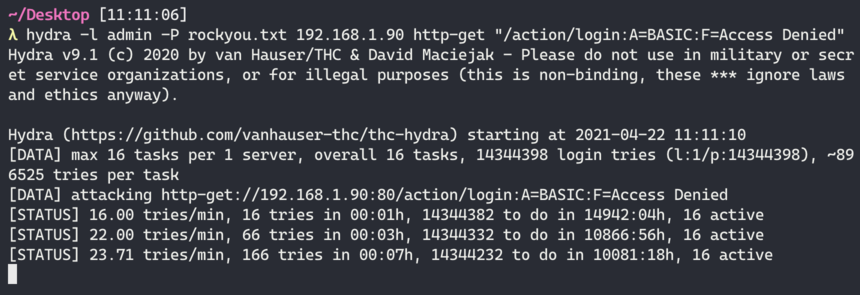
\includegraphics[width=\textwidth]{images/6-pentesting/hydra-results.png}
    \caption{The results of running a password attack.}
    \label{fig:hydra-password-attack}
\end{figure}

\subsection{Discussion}
The Hydra tool was only able to do around 23 requests per minute. Hydra is known to be very fast, so that is not the issue. One explanation for why this was so slow could be that the server rate-limits users. This is a common technique to protect against password attacks, if enough failed login attempts occur from a single IP the server would temporarily block or throttle it. However, there are signs indicating that this is not the case. For example, accessing the main web page slows down tremendously while performing the attack. Initially, it had around a \textit{16ms} response time, which increased to over \textit{17 seconds} during the attack. This was even confirmed on another computer, indicating that the main panel has not implemented any form rate-limiting per IP address. Presumably, the system is instead simply resource-bound and cannot serve requests at a faster rate. Given the hardware of the system, this is not unlikely. The CPU is most likely not that powerful, as is often the case in \gls{IOT} systems.

Due to the main panel not being able to serve more than 23 requests per minute, this type of attack is not feasible. For example, running a brute force attack, testing just all possible eight-character passwords, would take well over a hundred thousand years. A well-crafted dictionary attack could perhaps be effective, even at these slow speeds. However, there is some indication that the password might be just a random string of characters, given that the default password cited in the user manual is \texttt{cX+HsA*7F1}. If that is the case then a brute force technique is the only possibility. For these reasons, the attack was deemed unfeasible and not pursued further.
